\part[20] Let $G$ be the graph that is obtained from the $6$-vertex cycle on vertices $u_1, \ldots, u_6$ after adding six new vertices $v_1, \ldots v_6$ with edges $u_iv_i$ for $i \in \{1,2,3,4,5,6\}$. Determine the treewidth of $G$ and prove also that $G$ has clique-width at most $4$.

\begin{solution}
    Consider the graph $\sunlet$ (shown below) as defined in the question. 
    \begin{center}
        \vspace{0.5em}
        \begin{tikzpicture}
            \node[main] (1) {}; 
            \node[main] (11) [above of=1] {}; 
            \node[main] (2) [right of=1] {}; 
            \node[main] (22) [above of=2] {}; 
            \node[main] (3) [below right of=2] {}; 
            \node[main] (33) [right of=3] {}; 
            \node[main] (4) [below left of=3]{}; 
            \node[main] (44) [below of=4] {}; 
            \node[main] (5) [left of=4] {}; 
            \node[main] (55) [below of=5] {}; 
            \node[main] (6) [above left of=5] {}; 
            \node[main] (66) [left of=6] {}; 
            \draw (1) -- (2) -- (3) -- (4) -- (5) -- (6) -- (1);
            \draw (1) -- (11);
            \draw (2) -- (22);
            \draw (3) -- (33);
            \draw (4) -- (44);
            \draw (5) -- (55);
            \draw (6) -- (66);
        \end{tikzpicture}
        \vspace{0.5em}
    \end{center}
    
    A connected graph with at least two vertices has treewidth 1 if and only if it is a tree, thus $\tw(\sunlet) > 1$. We may define the treewidth of $G$, $\tw(G)$, as one less than smallest clique number of the chordal graphs containing $G$ as a spanning subgraph. Consider the following triangulation of $\sunlet$. 

    \begin{center}
        \vspace{0.5em}
        \begin{tikzpicture}
            \node[main] (1) {}; 
            \node[main] (11) [above of=1] {}; 
            \node[main] (2) [right of=1] {}; 
            \node[main] (22) [above of=2] {}; 
            \node[main] (3) [below right of=2] {}; 
            \node[main] (33) [right of=3] {}; 
            \node[main] (4) [below left of=3]{}; 
            \node[main] (44) [below of=4] {}; 
            \node[main] (5) [left of=4] {}; 
            \node[main] (55) [below of=5] {}; 
            \node[main] (6) [above left of=5] {}; 
            \node[main] (66) [left of=6] {}; 
            \draw (1) -- (2) -- (3) -- (4) -- (5) -- (6) -- (1);
            \draw (1) -- (11);
            \draw (2) -- (22);
            \draw (3) -- (33);
            \draw (4) -- (44);
            \draw (5) -- (55);
            \draw (6) -- (66);
            \draw (1) -- (4);
            \draw (1) -- (3);
            \draw (1) -- (5);
        \end{tikzpicture}
        \vspace{0.5em}
    \end{center}

    This is graph is chordal, contains $G$ as a spanning subgraph, and has clique number $3$. Thus, $\tw(\sunlet) \leq 2$. But we have seen that $\tw(\sunlet) > 1$, so $\tw(\sunlet) = 2$. 

    The bound $\cw(\sunlet) \leq 3 \cdot 2^{\tw(\sunlet) - 1} = 6$ is too high for this question, so we move to a constructive proof of the bound $4$ given. This diagram is to be read left to right.

    \begin{center}
        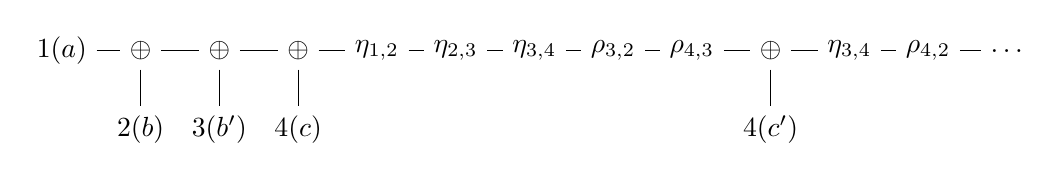
\begin{tikzpicture}[node distance={10mm}]
            \node (1) {$1(a)$};
            \node (2) [right of=1] {$\oplus$};
            \node (222) [below of=2] {$2(b)$};
            \node (3) [right of=2] {$\oplus$};
            \node (333) [below of=3] {$3(b')$};
            \node (4) [right of=3] {$\oplus$};
            \node (444) [below of=4] {$4(c)$};
            \node (5) [right of=4] {$\eta_{1,2}$};
            \node (6) [right of=5] {$\eta_{2,3}$};
            \node (7) [right of=6] {$\eta_{3,4}$};
            \node (8) [right of=7] {$\rho_{3,2}$};
            \node (9) [right of=8] {$\rho_{4,3}$};
            \node (10) [right of=9] {$\oplus$};
            \node (100) [below of=10] {$4(c')$};
            \node (11) [right of=10] {$\eta_{3,4}$};
            \node (12) [right of=11] {$\rho_{4,2}$};
            \node (13) [right of=12] {$\ldots$};
            \draw (1) -- (2) -- (3) -- (4) -- (5) -- (6) -- (7) -- (8) -- (9) -- (10) -- (11) -- (12) -- (12) -- (13); 
            \draw (2) -- (222) (3) -- (333) (4) -- (444) (10) -- (100);
        \end{tikzpicture}

        \vspace{1em}

        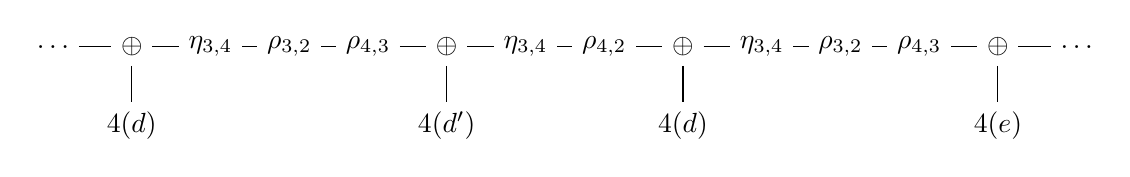
\begin{tikzpicture}[node distance={10mm}]
            \node (0) {$\ldots$};
            \node (13) [right of=0] {$\oplus$};
            \node (133) [below of=13] {$4(d)$};
            \node (14) [right of=13] {$\eta_{3,4}$};
            \node (15) [right of=14] {$\rho_{3,2}$};
            \node (16) [right of=15] {$\rho_{4,3}$};
            \node (17) [right of=16] {$\oplus$};
            \node (177) [below of=17] {$4(d')$};
            \node (18) [right of=17] {$\eta_{3,4}$};
            \node (19) [right of=18] {$\rho_{4,2}$};
            \node (20) [right of=19] {$\oplus$};
            \node (200) [below of=20] {$4(d)$};
            \node (21) [right of=20] {$\eta_{3,4}$};
            \node (22) [right of=21] {$\rho_{3,2}$};
            \node (23) [right of=22] {$\rho_{4,3}$};
            \node (24) [right of=23] {$\oplus$};
            \node (244) [below of=24] {$4(e)$};
            \node (25) [right of=24] {$\ldots$};
            \draw (0) -- (13) -- (14) -- (15) -- (16) -- (17) -- (18) -- (19) -- (20) -- (21) -- (22) -- (23) -- (24) -- (25);
            \draw (13) -- (133) (17) -- (177) (20) -- (200) (24) -- (244);
        \end{tikzpicture}

        \vspace{1em}

        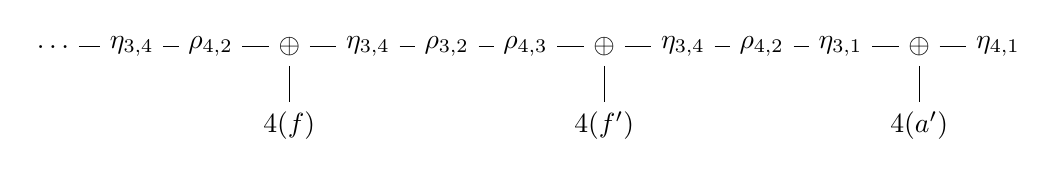
\begin{tikzpicture}[node distance={10mm}]
            \node (0) {$\ldots$};
            \node (25) [right of=0] {$\eta_{3,4}$};
            \node (26) [right of=25] {$\rho_{4,2}$};
            \node (27) [right of=26] {$\oplus$};
            \node (277) [below of=27] {$4(f)$};
            \node (28) [right of=27] {$\eta_{3,4}$};
            \node (29) [right of=28] {$\rho_{3,2}$};
            \node (30) [right of=29] {$\rho_{4,3}$};
            \node (31) [right of=30] {$\oplus$};
            \node (311) [below of=31] {$4(f')$};
            \node (32) [right of=31] {$\eta_{3,4}$};
            \node (33) [right of=32] {$\rho_{4,2}$};
            \node (34) [right of=33] {$\eta_{3,1}$};
            \node (35) [right of=34] {$\oplus$};
            \node (355) [below of=35] {$4(a')$};
            \node (36) [right of=35] {$\eta_{4,1}$};
            \draw (0) -- (25) -- (26) -- (27) -- (28) -- (29) -- (30) -- (31) -- (32) -- (33) -- (34) -- (35) -- (36);
            \draw (27) -- (277) (31) -- (311) (35) -- (355);
        \end{tikzpicture}
    \end{center}
    Thus, in this $k$-expression we use at most $4$ labels, and it constructs $\sunlet$. Thus $\cw(\sunlet) \leq 4$ as required.
\end{solution}